\hypertarget{libphonefirewall_8h}{
\section{libphonefirewall.h File Reference}
\label{libphonefirewall_8h}\index{libphonefirewall.h@{libphonefirewall.h}}
}
API of the phone firewall. 



This graph shows which files directly or indirectly include this file:\nopagebreak
\begin{figure}[H]
\begin{center}
\leavevmode
\includegraphics[width=104pt]{libphonefirewall_8h__dep__incl}
\end{center}
\end{figure}
\subsection*{Data Structures}
\begin{CompactItemize}
\item 
struct \hyperlink{structentry}{entry}
\begin{CompactList}\small\item\em Includes all informations for an \hyperlink{structentry}{entry}. \item\end{CompactList}\end{CompactItemize}
\subsection*{Defines}
\begin{CompactItemize}
\item 
\#define \hyperlink{libphonefirewall_8h_f0f2173e3b202ddf5756531b4471dcb2}{MAX\_\-LINE\_\-LENGTH}~512
\item 
\#define \hyperlink{libphonefirewall_8h_6265f3115ead4b41b74ad4b8fe53a801}{PRIO\_\-ALL}~-999
\end{CompactItemize}
\subsection*{Functions}
\begin{CompactItemize}
\item 
int \hyperlink{libphonefirewall_8h_36847ed3459e2a89038772ece42a017d}{add\_\-blacklist\_\-entry} (int country\_\-code, int area\_\-code, unsigned long long number, char $\ast$name, char $\ast$reason, int priority)
\item 
int \hyperlink{libphonefirewall_8h_e6c567f38aaa0eaa9db3eb13e32cdbbd}{rm\_\-blacklist\_\-entry} (unsigned long long number)
\item 
char $\ast$ \hyperlink{libphonefirewall_8h_651cdd0245f20256305b40f13bb9df2d}{check\_\-blacklist\_\-entry} (int country\_\-code, int area\_\-code, unsigned long long number, int priority)
\item 
int \hyperlink{libphonefirewall_8h_eec16cb88eb546b1a2490e6716d75f8b}{add\_\-whitelist\_\-entry} (int country\_\-code, int area\_\-code, unsigned long long number, char $\ast$name, char $\ast$reason, int priority)
\item 
struct \hyperlink{structentry}{entry} $\ast$ \hyperlink{libphonefirewall_8h_04b29323de592cc442250d7c952213de}{get\_\-blacklist\_\-entry\_\-by\_\-name} (char $\ast$name)
\item 
struct \hyperlink{structentry}{entry} $\ast$ \hyperlink{libphonefirewall_8h_80b7f603605d9ea57e83847bed7840f3}{get\_\-blacklist\_\-entry\_\-by\_\-number} (int country\_\-code, int area\_\-code, unsigned long long number)
\item 
int \hyperlink{libphonefirewall_8h_e8a4ee30cf26b05a55680dc3a972f1a4}{rm\_\-whitelist\_\-entry} (unsigned long long number)
\item 
char $\ast$ \hyperlink{libphonefirewall_8h_032c45d6c7830492ddeaa8cabfc845c3}{check\_\-whitelist\_\-entry} (int country\_\-code, int area\_\-code, unsigned long long number, int priority)
\item 
struct \hyperlink{structentry}{entry} $\ast$ \hyperlink{libphonefirewall_8h_f7f20dcd932db52fce6beac057995533}{get\_\-whitelist\_\-entry\_\-by\_\-name} (char $\ast$name)
\item 
struct \hyperlink{structentry}{entry} $\ast$ \hyperlink{libphonefirewall_8h_9569cf612525d13ec3443a5df88afe78}{get\_\-whitelist\_\-entry\_\-by\_\-number} (int country\_\-code, int area\_\-code, unsigned long long number)
\end{CompactItemize}


\subsection{Detailed Description}
API of the phone firewall. 

\begin{Desc}
\item[Author:]Alex Oberhauser\end{Desc}
The header file of the Phone Firewall. Blocks or accepts incoming phone calls, so it's possible to prevent disturbing phone calls. Provides a API which can used by other application to build nice programs.

Implemented for the OpenMoko framework. 

Definition in file \hyperlink{libphonefirewall_8h-source}{libphonefirewall.h}.

\subsection{Define Documentation}
\hypertarget{libphonefirewall_8h_f0f2173e3b202ddf5756531b4471dcb2}{
\index{libphonefirewall.h@{libphonefirewall.h}!MAX\_\-LINE\_\-LENGTH@{MAX\_\-LINE\_\-LENGTH}}
\index{MAX\_\-LINE\_\-LENGTH@{MAX\_\-LINE\_\-LENGTH}!libphonefirewall.h@{libphonefirewall.h}}
\subsubsection{\setlength{\rightskip}{0pt plus 5cm}\#define MAX\_\-LINE\_\-LENGTH~512}}
\label{libphonefirewall_8h_f0f2173e3b202ddf5756531b4471dcb2}




Definition at line 33 of file libphonefirewall.h.

Referenced by check\_\-blacklist\_\-entry(), and check\_\-whitelist\_\-entry().\hypertarget{libphonefirewall_8h_6265f3115ead4b41b74ad4b8fe53a801}{
\index{libphonefirewall.h@{libphonefirewall.h}!PRIO\_\-ALL@{PRIO\_\-ALL}}
\index{PRIO\_\-ALL@{PRIO\_\-ALL}!libphonefirewall.h@{libphonefirewall.h}}
\subsubsection{\setlength{\rightskip}{0pt plus 5cm}\#define PRIO\_\-ALL~-999}}
\label{libphonefirewall_8h_6265f3115ead4b41b74ad4b8fe53a801}




Definition at line 34 of file libphonefirewall.h.

Referenced by add\_\-blacklist\_\-entry(), add\_\-whitelist\_\-entry(), check\_\-blacklist\_\-entry(), and check\_\-whitelist\_\-entry().

\subsection{Function Documentation}
\hypertarget{libphonefirewall_8h_36847ed3459e2a89038772ece42a017d}{
\index{libphonefirewall.h@{libphonefirewall.h}!add\_\-blacklist\_\-entry@{add\_\-blacklist\_\-entry}}
\index{add\_\-blacklist\_\-entry@{add\_\-blacklist\_\-entry}!libphonefirewall.h@{libphonefirewall.h}}
\subsubsection{\setlength{\rightskip}{0pt plus 5cm}int add\_\-blacklist\_\-entry (int {\em country\_\-code}, int {\em area\_\-code}, unsigned long long {\em number}, char $\ast$ {\em name}, char $\ast$ {\em reason}, int {\em priority})}}
\label{libphonefirewall_8h_36847ed3459e2a89038772ece42a017d}


Add a number to the blacklist. The number will be blocked after that.

\begin{Desc}
\item[Parameters:]
\begin{description}
\item[{\em country\_\-code}]The country code (for example 39 for Italy, 43 for Austria, and so one) \item[{\em area\_\-code}]The area code which indicates your mobile operator. \item[{\em number}]The telephone number of the person (without country and area code. \item[{\em name}]The name of the person. \item[{\em reason}]Why you have blocked this person. \item[{\em priority}]Gives the \hyperlink{structentry}{entry} a priority. 0 is standard. If the priority is higher the value will be also blocked/accepted if a higher priority is choosen. \par
 The value \char`\"{}PRIO\_\-ALL\char`\"{} stands for all priorities.\end{description}
\end{Desc}
\begin{Desc}
\item[Returns:]If all goes well 0 (zero) otherwise an errno code. \end{Desc}


Definition at line 40 of file phonefirewall\_\-administration.c.

References BLACKLIST\_\-PREFIX, check\_\-blacklist\_\-entry(), DELIM, filename, PRIO\_\-ALL, and set\_\-filename().

Here is the call graph for this function:\nopagebreak
\begin{figure}[H]
\begin{center}
\leavevmode
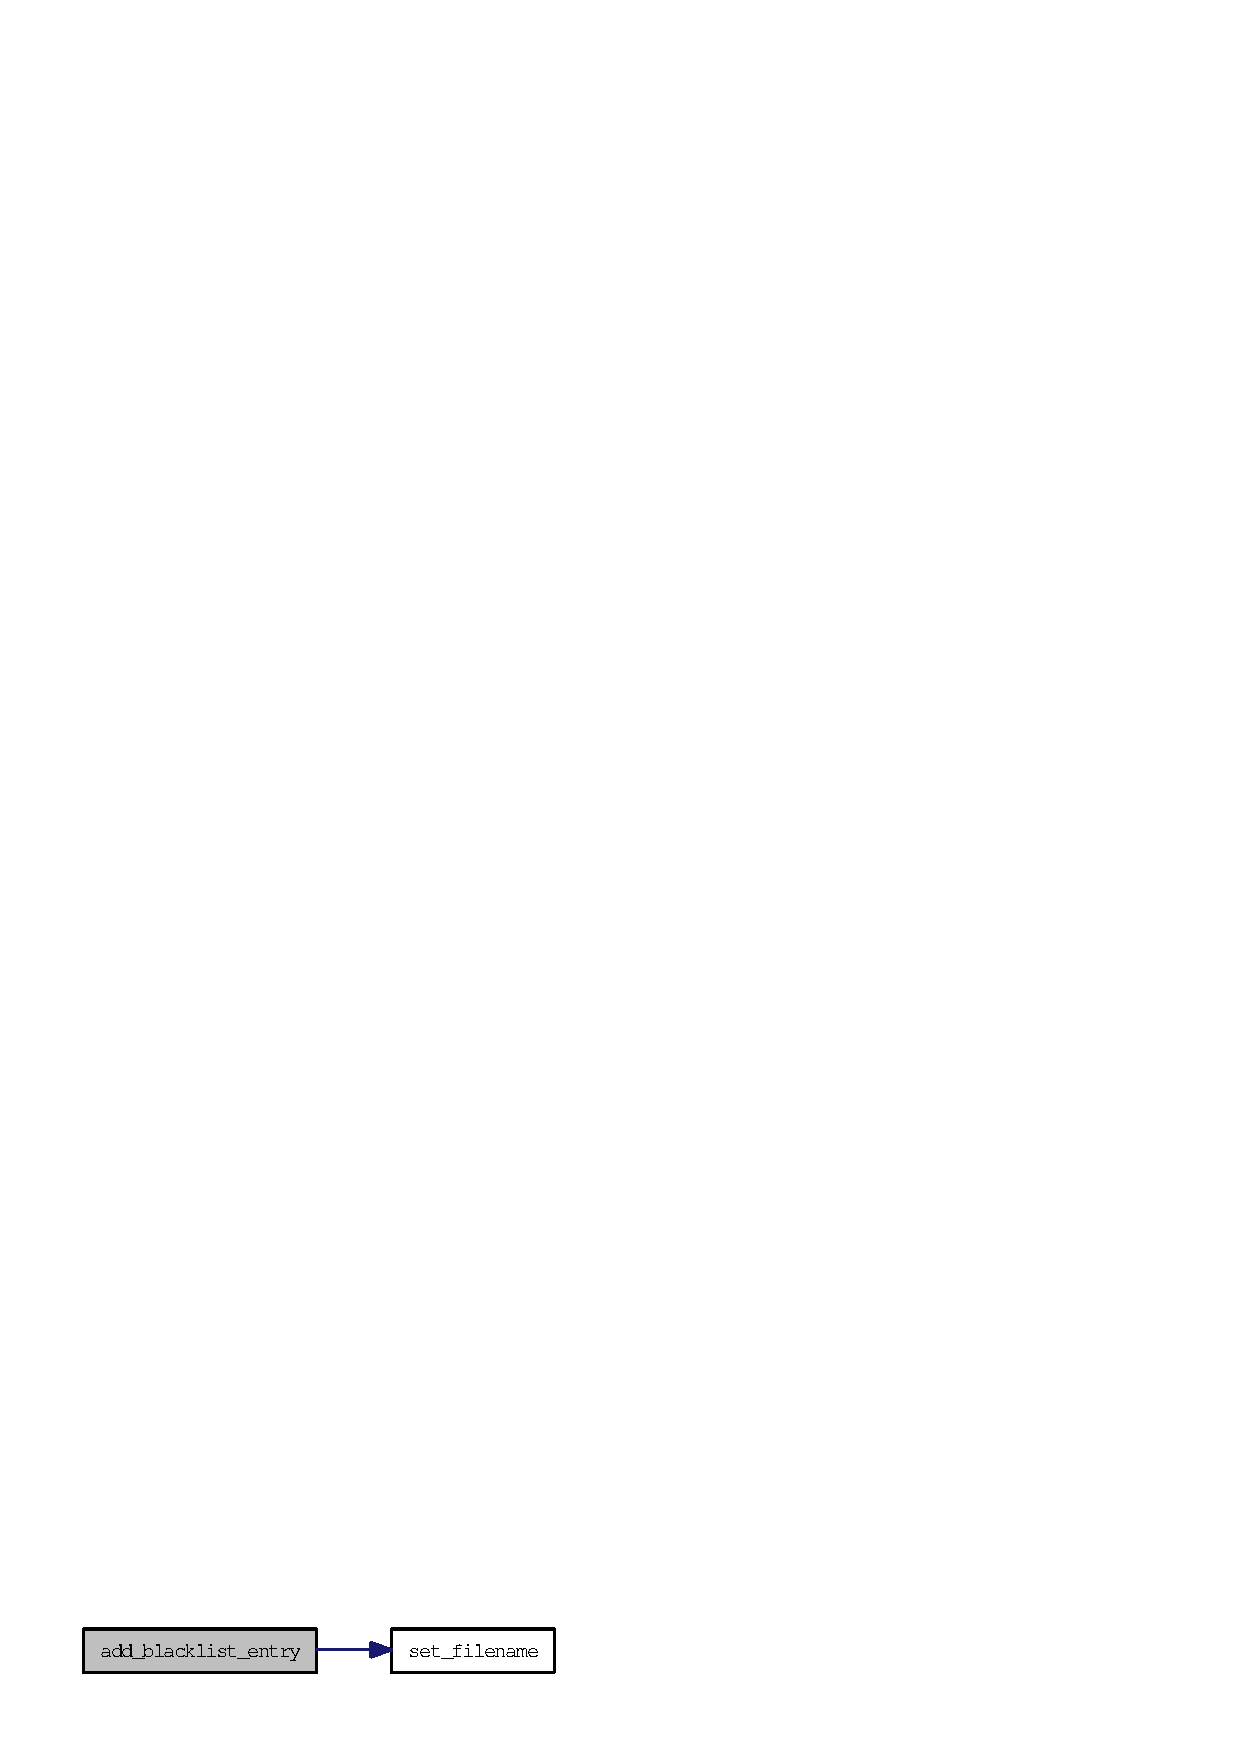
\includegraphics[width=215pt]{libphonefirewall_8h_36847ed3459e2a89038772ece42a017d_cgraph}
\end{center}
\end{figure}
\hypertarget{libphonefirewall_8h_eec16cb88eb546b1a2490e6716d75f8b}{
\index{libphonefirewall.h@{libphonefirewall.h}!add\_\-whitelist\_\-entry@{add\_\-whitelist\_\-entry}}
\index{add\_\-whitelist\_\-entry@{add\_\-whitelist\_\-entry}!libphonefirewall.h@{libphonefirewall.h}}
\subsubsection{\setlength{\rightskip}{0pt plus 5cm}int add\_\-whitelist\_\-entry (int {\em country\_\-code}, int {\em area\_\-code}, unsigned long long {\em number}, char $\ast$ {\em name}, char $\ast$ {\em reason}, int {\em priority})}}
\label{libphonefirewall_8h_eec16cb88eb546b1a2490e6716d75f8b}


Add a number to the whitelist. The number will be accepted after that.

\begin{Desc}
\item[Parameters:]
\begin{description}
\item[{\em country\_\-code}]The country code (for example 39 for Italy, 43 for Austria, and so one) \item[{\em area\_\-code}]The area code which indicates your mobile operator. \item[{\em number}]The telephone number of the person (without country and area code. \item[{\em name}]The name of the person. \item[{\em reason}]Why you have blocked this person. \item[{\em priority}]Gives the \hyperlink{structentry}{entry} a priority. 0 is standard. If the priority is higher the value will be also blocked/accepted if a higher priority is choosen.\par
 The value \char`\"{}PRIO\_\-ALL\char`\"{} stands for all priorities.\end{description}
\end{Desc}
\begin{Desc}
\item[Returns:]If all goes well 0 (zero) otherwise an errno code. \end{Desc}


Definition at line 57 of file phonefirewall\_\-administration.c.

References check\_\-whitelist\_\-entry(), DELIM, filename, PRIO\_\-ALL, set\_\-filename(), and WHITELIST\_\-PREFIX.

Here is the call graph for this function:\nopagebreak
\begin{figure}[H]
\begin{center}
\leavevmode
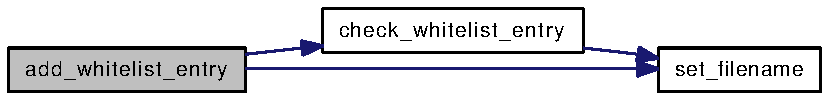
\includegraphics[width=217pt]{libphonefirewall_8h_eec16cb88eb546b1a2490e6716d75f8b_cgraph}
\end{center}
\end{figure}
\hypertarget{libphonefirewall_8h_651cdd0245f20256305b40f13bb9df2d}{
\index{libphonefirewall.h@{libphonefirewall.h}!check\_\-blacklist\_\-entry@{check\_\-blacklist\_\-entry}}
\index{check\_\-blacklist\_\-entry@{check\_\-blacklist\_\-entry}!libphonefirewall.h@{libphonefirewall.h}}
\subsubsection{\setlength{\rightskip}{0pt plus 5cm}char$\ast$ check\_\-blacklist\_\-entry (int {\em country\_\-code}, int {\em area\_\-code}, unsigned long long {\em number}, int {\em priority})}}
\label{libphonefirewall_8h_651cdd0245f20256305b40f13bb9df2d}


Checks if a number is on the blacklist.

\begin{Desc}
\item[Parameters:]
\begin{description}
\item[{\em country\_\-code}]The country code (for example 39 for Italy, 43 for Austria, and so one) \item[{\em area\_\-code}]The area code which indicates your mobile operator. \item[{\em number}]The telephone number of the person (without country and area code. \item[{\em priority}]Gives the \hyperlink{structentry}{entry} a priority. 0 is standard. If the priority is higher the value will be also blocked/accepted if a higher priority is choosen.\par
 The value \char`\"{}PRIO\_\-ALL\char`\"{} stands for all priorities.\end{description}
\end{Desc}
\begin{Desc}
\item[Returns:]If noting is found NULL, otherwise the number. \end{Desc}


Definition at line 81 of file phonefirewall\_\-administration.c.

References BLACKLIST\_\-PREFIX, DELIM, filename, MAX\_\-LINE\_\-LENGTH, PRIO\_\-ALL, and set\_\-filename().

Referenced by add\_\-blacklist\_\-entry().

Here is the call graph for this function:\nopagebreak
\begin{figure}[H]
\begin{center}
\leavevmode
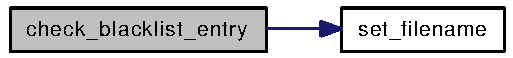
\includegraphics[width=141pt]{libphonefirewall_8h_651cdd0245f20256305b40f13bb9df2d_cgraph}
\end{center}
\end{figure}


Here is the caller graph for this function:\nopagebreak
\begin{figure}[H]
\begin{center}
\leavevmode
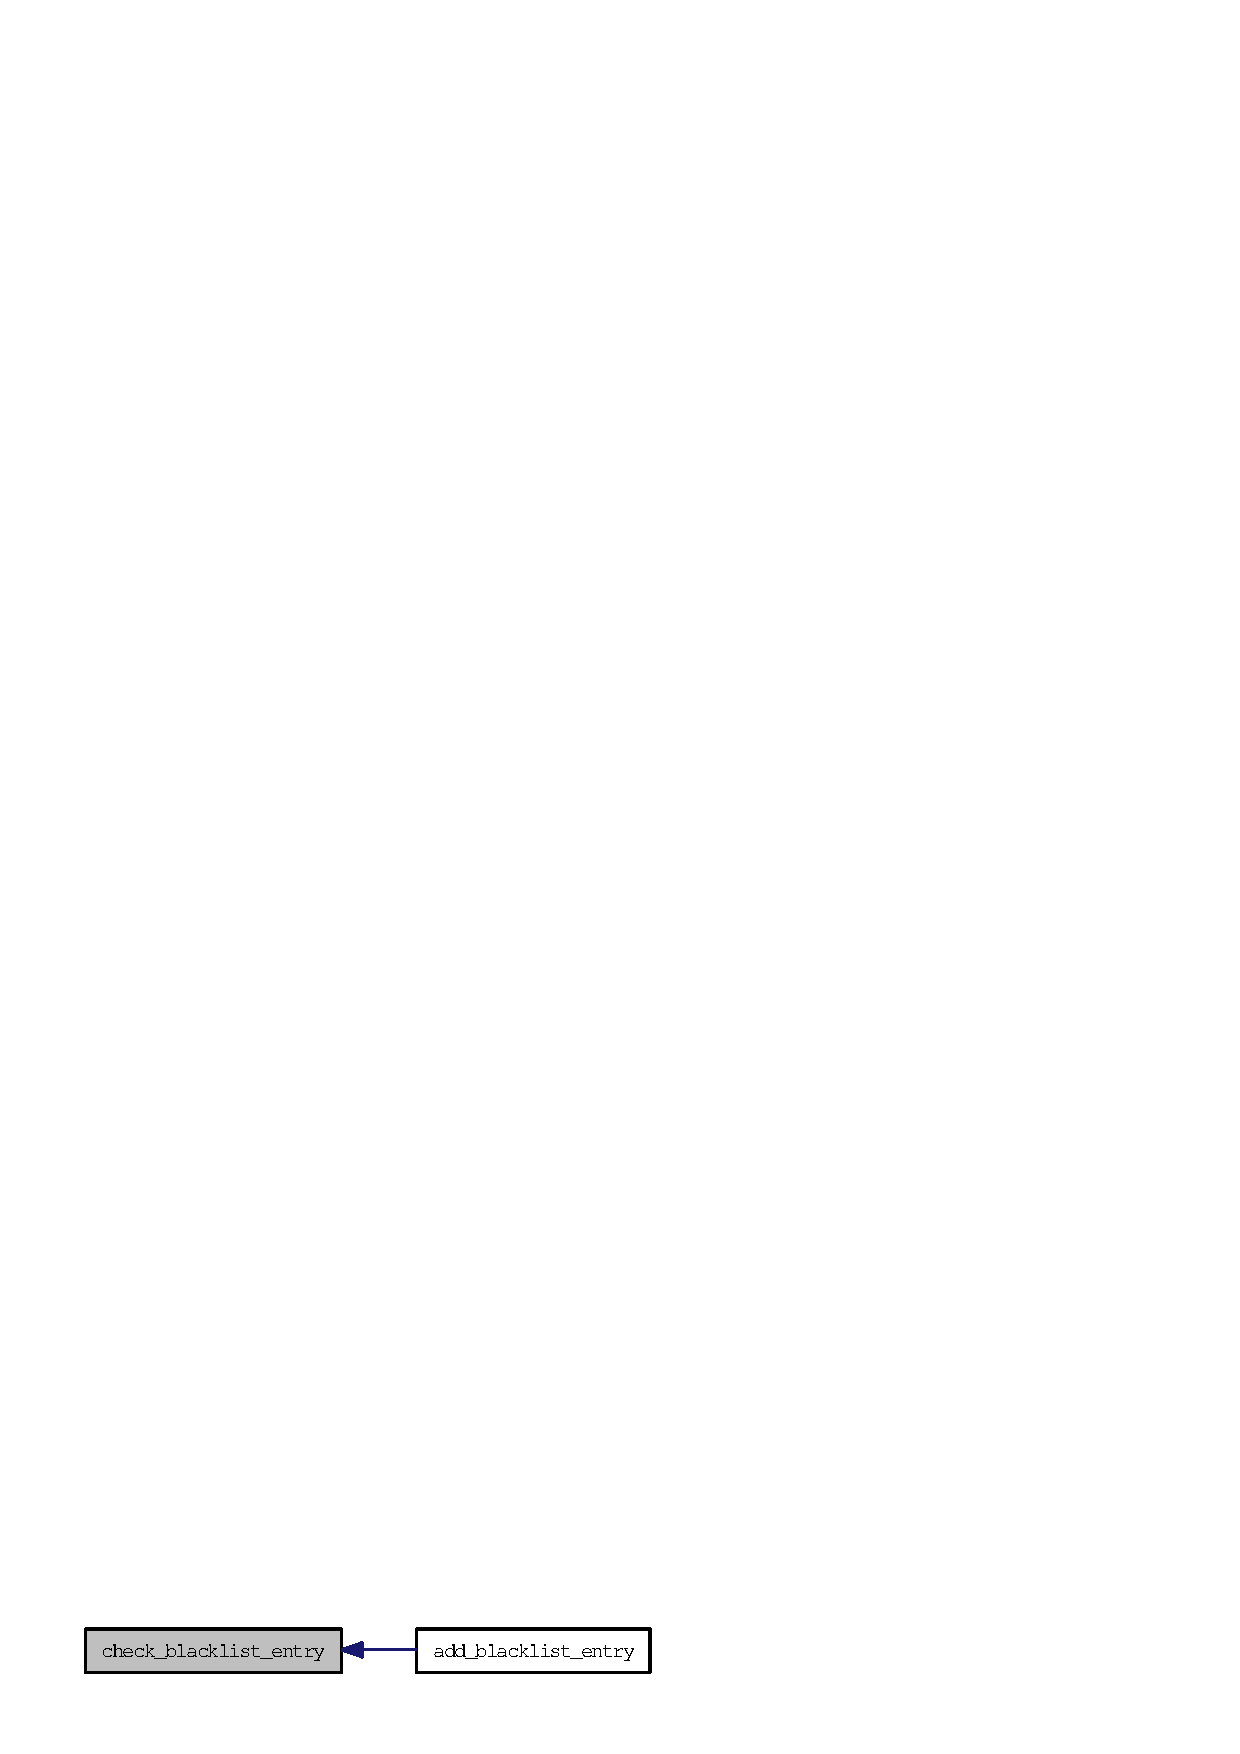
\includegraphics[width=158pt]{libphonefirewall_8h_651cdd0245f20256305b40f13bb9df2d_icgraph}
\end{center}
\end{figure}
\hypertarget{libphonefirewall_8h_032c45d6c7830492ddeaa8cabfc845c3}{
\index{libphonefirewall.h@{libphonefirewall.h}!check\_\-whitelist\_\-entry@{check\_\-whitelist\_\-entry}}
\index{check\_\-whitelist\_\-entry@{check\_\-whitelist\_\-entry}!libphonefirewall.h@{libphonefirewall.h}}
\subsubsection{\setlength{\rightskip}{0pt plus 5cm}char$\ast$ check\_\-whitelist\_\-entry (int {\em country\_\-code}, int {\em area\_\-code}, unsigned long long {\em number}, int {\em priority})}}
\label{libphonefirewall_8h_032c45d6c7830492ddeaa8cabfc845c3}


Checks if a number is on the whitelist.

\begin{Desc}
\item[Parameters:]
\begin{description}
\item[{\em country\_\-code}]The country code (for example 39 for Italy, 43 for Austria, and so one) \item[{\em area\_\-code}]The area code which indicates your mobile operator. \item[{\em number}]The telephone number of the person (without country and area code. \item[{\em priority}]Gives the \hyperlink{structentry}{entry} a priority. 0 is standard. If the priority is higher the value will be also blocked/accepted if a higher priority is choosen.\par
 The value \char`\"{}PRIO\_\-ALL\char`\"{} stands for all priorities.\end{description}
\end{Desc}
\begin{Desc}
\item[Returns:]If noting is found NULL, otherwise the number. \end{Desc}


Definition at line 121 of file phonefirewall\_\-administration.c.

References DELIM, filename, MAX\_\-LINE\_\-LENGTH, PRIO\_\-ALL, set\_\-filename(), and WHITELIST\_\-PREFIX.

Referenced by add\_\-whitelist\_\-entry().

Here is the call graph for this function:\nopagebreak
\begin{figure}[H]
\begin{center}
\leavevmode
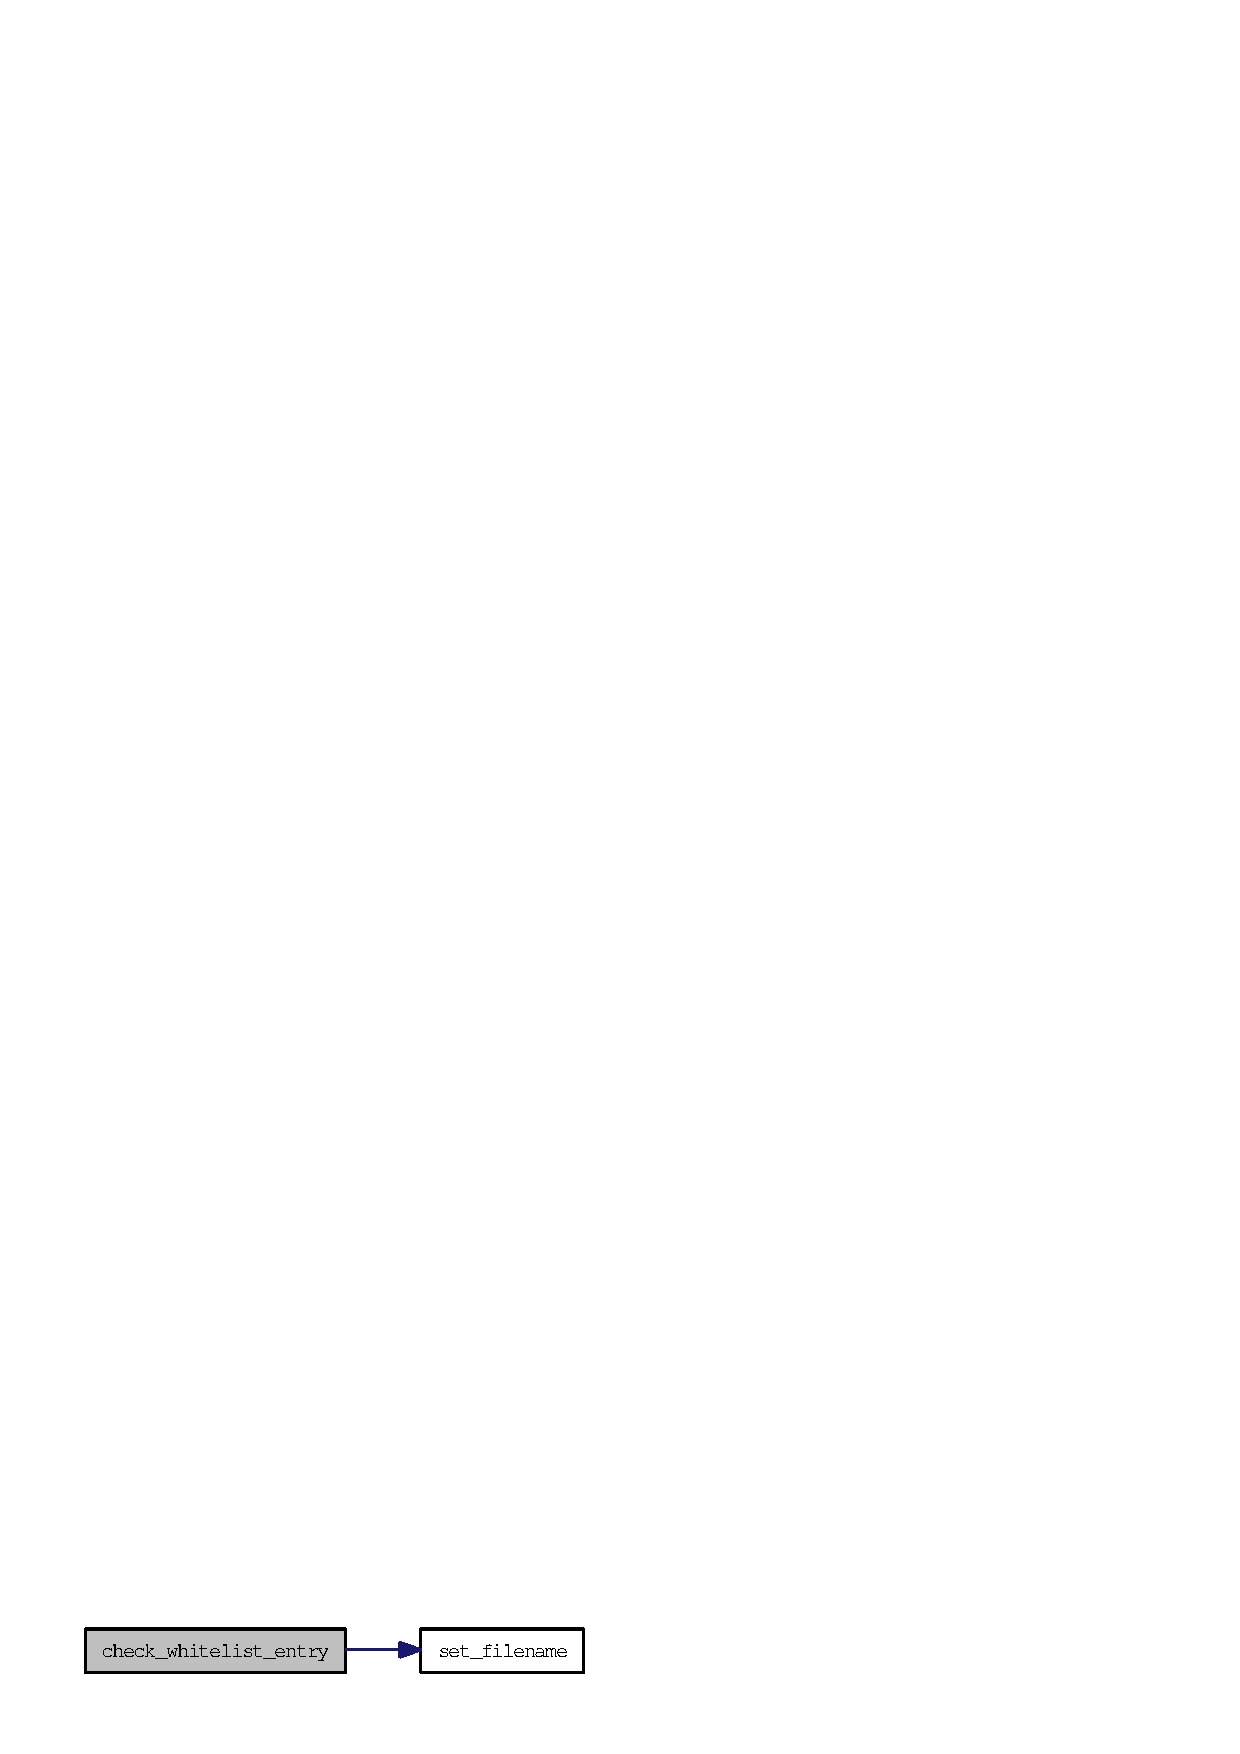
\includegraphics[width=142pt]{libphonefirewall_8h_032c45d6c7830492ddeaa8cabfc845c3_cgraph}
\end{center}
\end{figure}


Here is the caller graph for this function:\nopagebreak
\begin{figure}[H]
\begin{center}
\leavevmode
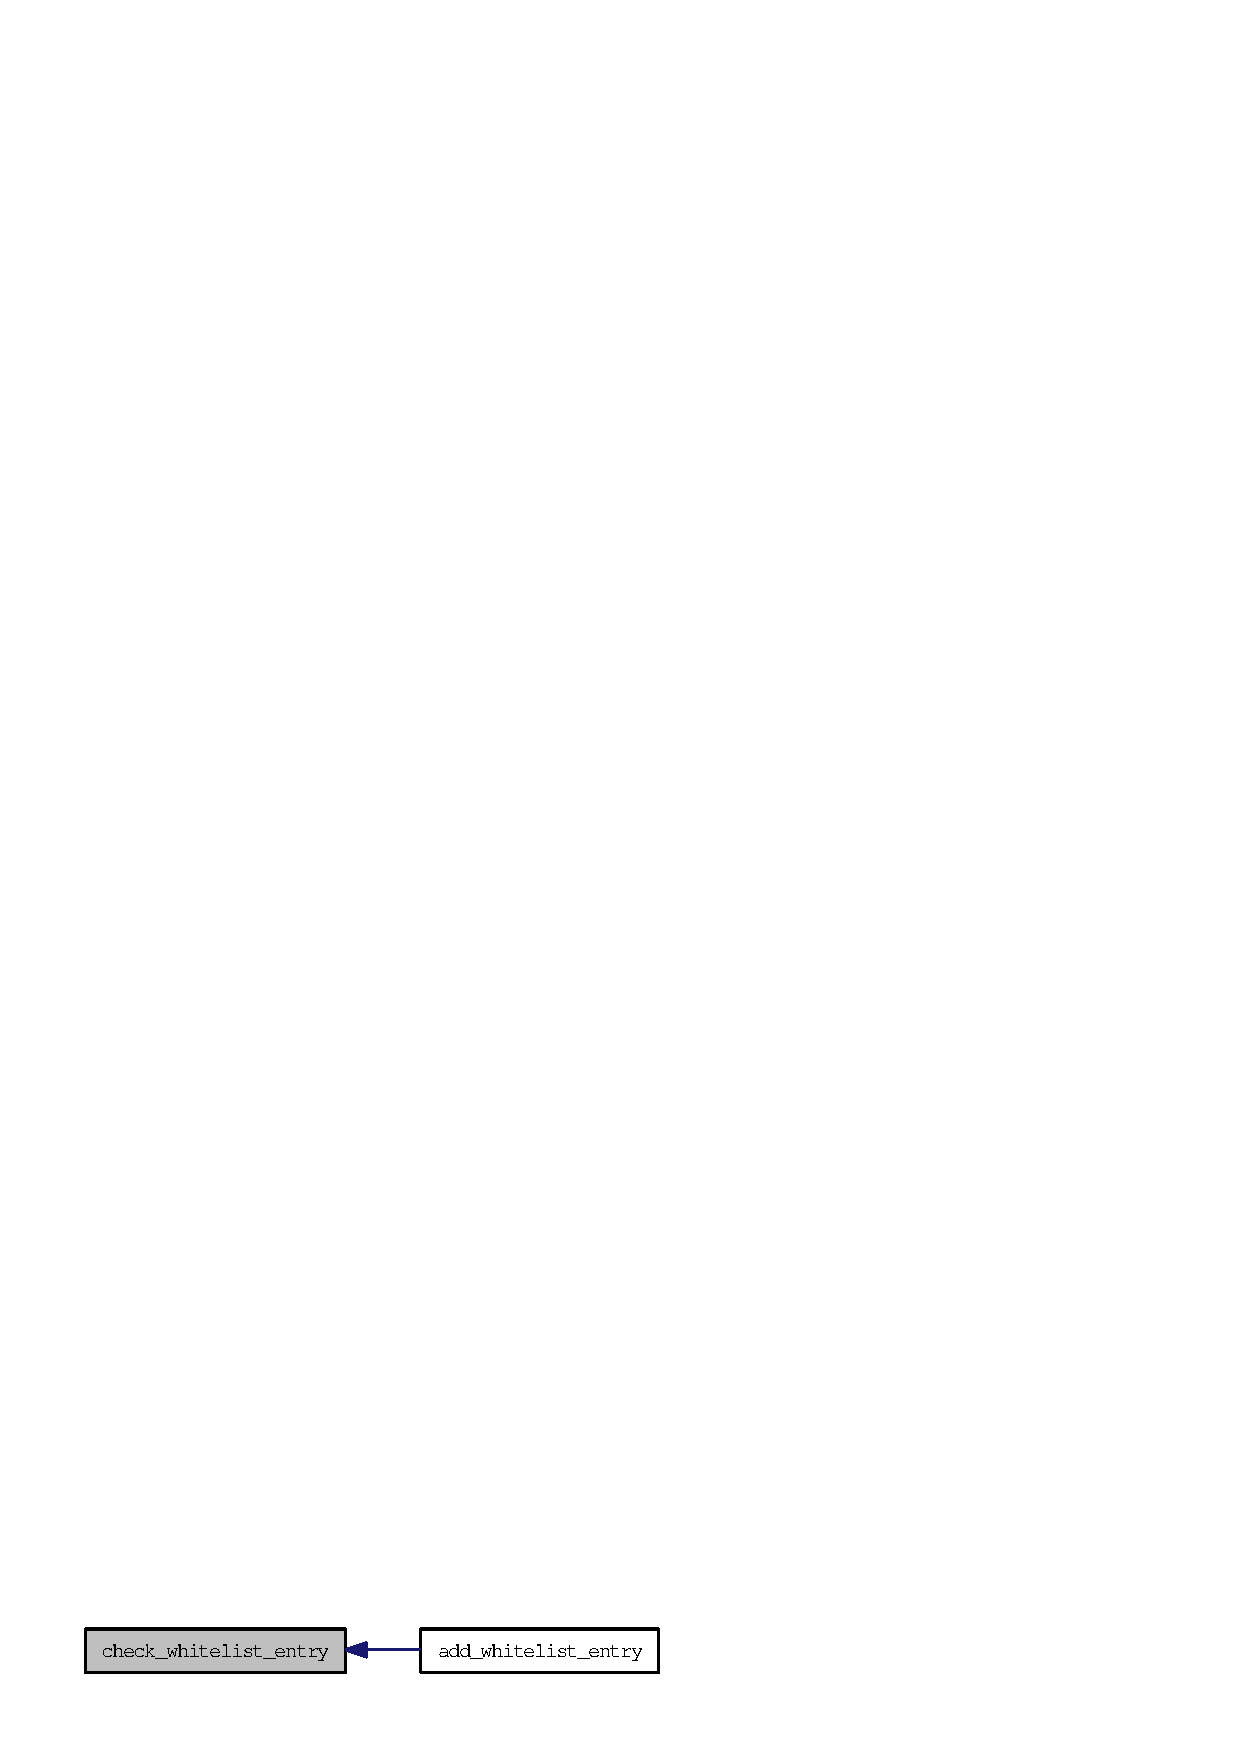
\includegraphics[width=160pt]{libphonefirewall_8h_032c45d6c7830492ddeaa8cabfc845c3_icgraph}
\end{center}
\end{figure}
\hypertarget{libphonefirewall_8h_04b29323de592cc442250d7c952213de}{
\index{libphonefirewall.h@{libphonefirewall.h}!get\_\-blacklist\_\-entry\_\-by\_\-name@{get\_\-blacklist\_\-entry\_\-by\_\-name}}
\index{get\_\-blacklist\_\-entry\_\-by\_\-name@{get\_\-blacklist\_\-entry\_\-by\_\-name}!libphonefirewall.h@{libphonefirewall.h}}
\subsubsection{\setlength{\rightskip}{0pt plus 5cm}struct {\bf entry}$\ast$ get\_\-blacklist\_\-entry\_\-by\_\-name (char $\ast$ {\em name})\hspace{0.3cm}{\tt  \mbox{[}read\mbox{]}}}}
\label{libphonefirewall_8h_04b29323de592cc442250d7c952213de}


Search a entrie by name.

\begin{Desc}
\item[Parameters:]
\begin{description}
\item[{\em name}]The name of the person which is blocked.\end{description}
\end{Desc}
\begin{Desc}
\item[Returns:]\hyperlink{structentry}{entry} Returns the found \hyperlink{structentry}{entry}. \end{Desc}
\hypertarget{libphonefirewall_8h_80b7f603605d9ea57e83847bed7840f3}{
\index{libphonefirewall.h@{libphonefirewall.h}!get\_\-blacklist\_\-entry\_\-by\_\-number@{get\_\-blacklist\_\-entry\_\-by\_\-number}}
\index{get\_\-blacklist\_\-entry\_\-by\_\-number@{get\_\-blacklist\_\-entry\_\-by\_\-number}!libphonefirewall.h@{libphonefirewall.h}}
\subsubsection{\setlength{\rightskip}{0pt plus 5cm}struct {\bf entry}$\ast$ get\_\-blacklist\_\-entry\_\-by\_\-number (int {\em country\_\-code}, int {\em area\_\-code}, unsigned long long {\em number})\hspace{0.3cm}{\tt  \mbox{[}read\mbox{]}}}}
\label{libphonefirewall_8h_80b7f603605d9ea57e83847bed7840f3}


Search a entrie by number (country code + area code + number).

\begin{Desc}
\item[Parameters:]
\begin{description}
\item[{\em country\_\-code}]The country code (for example 39 for Italy, 43 for Austria, and so one) \item[{\em area\_\-code}]The area code which indicates your mobile operator. \item[{\em number}]The telephone number of the person (without country and area code.\end{description}
\end{Desc}
\begin{Desc}
\item[Returns:]\hyperlink{structentry}{entry} Returns the found \hyperlink{structentry}{entry}. \end{Desc}
\hypertarget{libphonefirewall_8h_f7f20dcd932db52fce6beac057995533}{
\index{libphonefirewall.h@{libphonefirewall.h}!get\_\-whitelist\_\-entry\_\-by\_\-name@{get\_\-whitelist\_\-entry\_\-by\_\-name}}
\index{get\_\-whitelist\_\-entry\_\-by\_\-name@{get\_\-whitelist\_\-entry\_\-by\_\-name}!libphonefirewall.h@{libphonefirewall.h}}
\subsubsection{\setlength{\rightskip}{0pt plus 5cm}struct {\bf entry}$\ast$ get\_\-whitelist\_\-entry\_\-by\_\-name (char $\ast$ {\em name})\hspace{0.3cm}{\tt  \mbox{[}read\mbox{]}}}}
\label{libphonefirewall_8h_f7f20dcd932db52fce6beac057995533}


Search a entrie by name.

\begin{Desc}
\item[Parameters:]
\begin{description}
\item[{\em name}]The name of the person which is accepted.\end{description}
\end{Desc}
\begin{Desc}
\item[Returns:]\hyperlink{structentry}{entry} Returns the found \hyperlink{structentry}{entry}. \end{Desc}
\hypertarget{libphonefirewall_8h_9569cf612525d13ec3443a5df88afe78}{
\index{libphonefirewall.h@{libphonefirewall.h}!get\_\-whitelist\_\-entry\_\-by\_\-number@{get\_\-whitelist\_\-entry\_\-by\_\-number}}
\index{get\_\-whitelist\_\-entry\_\-by\_\-number@{get\_\-whitelist\_\-entry\_\-by\_\-number}!libphonefirewall.h@{libphonefirewall.h}}
\subsubsection{\setlength{\rightskip}{0pt plus 5cm}struct {\bf entry}$\ast$ get\_\-whitelist\_\-entry\_\-by\_\-number (int {\em country\_\-code}, int {\em area\_\-code}, unsigned long long {\em number})\hspace{0.3cm}{\tt  \mbox{[}read\mbox{]}}}}
\label{libphonefirewall_8h_9569cf612525d13ec3443a5df88afe78}


Search a entrie by number (country code + area code + number).

\begin{Desc}
\item[Parameters:]
\begin{description}
\item[{\em country\_\-code}]The country code (for example 39 for Italy, 43 for Austria, and so one) \item[{\em area\_\-code}]The area code which indicates your mobile operator. \item[{\em number}]The telephone number of the person (without country and area code.\end{description}
\end{Desc}
\begin{Desc}
\item[Returns:]\hyperlink{structentry}{entry} Returns the found \hyperlink{structentry}{entry}. \end{Desc}
\hypertarget{libphonefirewall_8h_e6c567f38aaa0eaa9db3eb13e32cdbbd}{
\index{libphonefirewall.h@{libphonefirewall.h}!rm\_\-blacklist\_\-entry@{rm\_\-blacklist\_\-entry}}
\index{rm\_\-blacklist\_\-entry@{rm\_\-blacklist\_\-entry}!libphonefirewall.h@{libphonefirewall.h}}
\subsubsection{\setlength{\rightskip}{0pt plus 5cm}int rm\_\-blacklist\_\-entry (unsigned long long {\em number})}}
\label{libphonefirewall_8h_e6c567f38aaa0eaa9db3eb13e32cdbbd}


Removes a blocked number from the blacklist.

\begin{Desc}
\item[Parameters:]
\begin{description}
\item[{\em number}]The number which will be deleted.\end{description}
\end{Desc}
\begin{Desc}
\item[Returns:]If all goes right 0, otherwise an error code. \end{Desc}


Definition at line 73 of file phonefirewall\_\-administration.c.\hypertarget{libphonefirewall_8h_e8a4ee30cf26b05a55680dc3a972f1a4}{
\index{libphonefirewall.h@{libphonefirewall.h}!rm\_\-whitelist\_\-entry@{rm\_\-whitelist\_\-entry}}
\index{rm\_\-whitelist\_\-entry@{rm\_\-whitelist\_\-entry}!libphonefirewall.h@{libphonefirewall.h}}
\subsubsection{\setlength{\rightskip}{0pt plus 5cm}int rm\_\-whitelist\_\-entry (unsigned long long {\em number})}}
\label{libphonefirewall_8h_e8a4ee30cf26b05a55680dc3a972f1a4}


Removes a accepted number from the whitelist.

\begin{Desc}
\item[Parameters:]
\begin{description}
\item[{\em number}]The number which will be deleted.\end{description}
\end{Desc}
\begin{Desc}
\item[Returns:]If all goes right 0, otherwise an error code. \end{Desc}


Definition at line 77 of file phonefirewall\_\-administration.c.